%!TEX root = ../thesis.tex
%Adding the above line, with the name of your base .tex file (in this case "thesis.tex") will allow you to compile the whole thesis even when working inside one of the chapter tex files
%: ----------------------- introduction file header -----------------------
\chapter{Introduction}
\label{chap:1}

The Sun has long been the focus of humanity's curiosity. Throughout history it has been the harbinger of new religions, philosophies, and sciences. It has changed our understanding of our place in the Universe and allowed us to push forward the frontiers of stellar astronomy. Although our understanding of the Sun is nowadays more advanced, the curiosity we hold for it has not changed since the very early humans.
Now, we understand the Sun is a star similar to any other in its class, currently going through a relatively unchanging 11 year cycle of activity that is extremely rich in physical complexity. The study of such complex phenomena has yielded immeasurable advances in many areas of physics such as spectroscopy, plasma physics, magnetohydrodynamics (MHD), particle physics, to name but a few. Although some of these sciences have grown over decades (or even centuries) they are still incomplete. I hope this theses, in some small way, will contribute to the continuing growth of these sciences and to the understanding of our nearest star.


%Here is the introduction of the thesis, complete with a few references  \citep{sagan1997demon, prothero2007evolution}.  Section \ref{sec:1} contains Equation \ref{eqn:1}, Section \ref{sec:2} has Figure \ref{fig:1} and Section \ref{sec:3} has Table \ref{tab:1}. Chapter \ref{chap:2} has pretty much nothing in it.

\section{The Sun}\label{sec:1}

The Sun is our nearest star, located $1.49\times10^6$\,km from Earth at the centre of our solar system. It is main sequence star of spectral class G2V, with a luminosity of $L_{\odot}=(3.84\pm 0.04)\times10^{26}$\,W, mass of $M_{\odot}=(1.989\pm0.0003)\times10^{30}$\,kg and radius of $R_{\odot}=(6.959\pm0.007)\times10^8$\,m \citep{foukal2004}. It was born approximately $4.6 \times 10^9$\,years ago when a giant molecular cloud underwent gravitational collapse and began hydrogen nuclear fusion at its centre (reference). The energy produced from this fusion resulted in enough pressure to counteract gravity and bring about a hydrostatic equilibrium ($\nabla P = -\rho g$) allowing the young star to reach a stability that is sustained today. It is estimated the Sun will maintain this stability for another 5 billion years, at which point, it will move off the main sequence and into the red giant phase. During this later part of its life, it will grow in size to 100 times its current radius and begin nuclear burning of heavier elements such as carbon and oxygen. Once carbon burning in the core is depleted it can no longer sustain nuclear fusion of heavier elements, resulting in a gravitational instability that will eventually lead to a stellar nova. This nova will result in the loss of the outer envelopes and ultimately the Sun's death, leaving behind a compact, dense white-dwarf.

Until such time, the Sun will remain on the main sequence in a regular state of hydrogen fusion in its core. The energy released during this process is the ultimate source of light and all energetic activity that we observe from Earth and beyond. Before we can understand how this energy manifests in the solar atmosphere as a variety of energetic phenomena, it is important to understand how the energy is generated inside the star and how it is transported through its interior.

\subsection{Solar Interior}\label{sec:10}

The source of the Sun's energy is nuclear fusion in the solar core. Temperatures as high as $15\times10^{6}$\,K allow four protons to fuse and become a helium nucleus i.e., $4\,^{1}$H$\rightarrow ^{4}$He\,+\,2e$^{+}+2\nu+2\gamma$, in a process known as the proton-proton or pp-chain. Here e$^+$, $\nu$, and $\gamma$ are a positron, neutrino, and gamma ray photon, respectively, resulting from fusion processes in the pp-chain. The solar core extends to approximately $0.25\,R_{\odot}$ from solar center where hydrogen burning (fusion) stops. Beyond this point, energy transport is dominated by photons scattering off of free particles. The transport of energy via radiation continues up to $\sim0.8\,R_{\odot}$, at which point the temperature is low enough such that neutral atoms form and radiation can no longer propagate freely due to the high opacity. Between $\sim0.8-1\,R_{\odot}$ the temperature gradient is large enough for convection to become the dominant mechanism for the transport of energy to the solar surface


\begin{figure}[!h]
\begin{center}
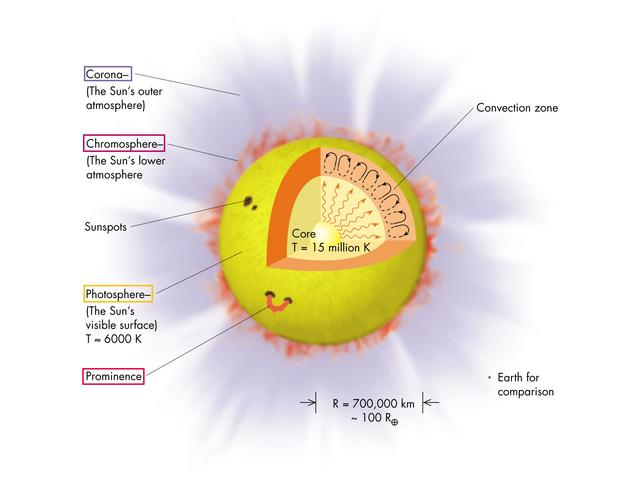
\includegraphics[trim = 0cm 0.5cm 0cm 0cm, width=1.0\textwidth]{images/solar_atmosphere}
\caption{The internal structure of the Sun, including the core, radiative zone, and convective zone.  Also shown is the structure of the its atmosphere, including the photosphere, chromosphere, and corona. The layers of the solar atmosphere are usually demarcated by temperature changes as height above the solar surface increases. The temperature ranges from $\sim$6000\,K in the photosphere to above 1\,MK in the corona.}
\label{fig:solar_atmosphere} 
\end{center}
\end{figure}



\subsection{Solar Dynamo and Magnetic Field}\label{sec:11}

\begin{figure}[!h]
\begin{center}
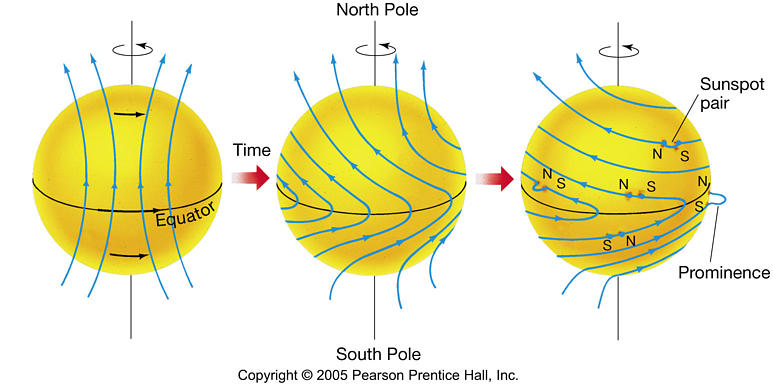
\includegraphics[]{images/Babcock}
\caption{Differential rotation and flux freezing result in the poloidal dipolar magnetic field, generated by dynamo action, to be dragged around in a toroidal direction, an action known as the omega effect. Buoyancy of the field lines results in them rising and twisting, known as the alpha effect, eventually surfacing to become bipolar fields that extend far into the corona.}
\label{fig:Babcock} 
\end{center}
\end{figure}

It is widely believed that the Sun's magnetic field is created by a dynamo action in a region between the radiative zone and the convection zone, known as the tachocline. Solar dynamo theory attempts to explain the observed 11 year magnetic activity cycle, where the the Sun's magnetic field starts as a poloidal dipolar structure and evolves to having a strong toroidal component, after which it returns to a poloidal field again. During these 11 years the Sun starts at minimum activity, reaches a maximum and returns to minimum again.

\citet{babcock1961} first explained this process by a mechanism involving differential rotation of the solar surface and interior. The equatorial rotation rate is faster than the rotation rate at higher latitudes. Because the magnetic field is frozen into the plasma, any flows in the solar interior will tend to drag the magnetic field along. By this effect, differential rotation tends to drag the field and wrap it around the Sun in a toroidal direction, this is known as the omega effect, see Figure~\ref{fig:Babcock}.

As the toroidal field builds up in the solar interior, sections of field lines build up in magnetic pressure resulting in a buoyancy of the field. The field slowly rises through the convection zone and eventually surfaces as a bipolar region that extends into the solar atmosphere. The presence of bipolar fields in the solar atmosphere and their slow build up over time to complex magnetic structures, known as active regions, ultimately leads to a variety of eruptive phenomena.



\subsection{Solar Atmosphere}\label{sec:12}

\subsubsection{Photosphere}\label{sec:121}

\begin{itemize}
\item Appearance, Granules, Sunspots.
\item Black Body Curve. Franhofer lines, H-alpha line, CaII H \& K, H$^{-}$ alines, Sodium D lines. 
\item Temperature, Density, Opacity.
\item Magnetic field strength
\end{itemize}

The most spectacular and energetic phenomena in our solar system have their origins in the solar atmosphere. This ever-changing and dynamic environment is a hotbed of activity giving rise to coronal mass ejections (CMEs), solar flares, and a host of plasma processes resulting in emission across the entire electromagnetic spectrum. To make sense of the phenomena we observe we must first have a basic understanding of solar atmospheric structure and the environment these processes take place in. Figure~\ref{fig:solar_atmosphere} is an illustration of the different layers of the solar interior, the solar surface and atmosphere. The visible surface of the Sun is known as the photosphere. It is demarcated where optical depth becomes unity for a wavelength of 5000\,\AA\ or $\tau_{5000}=1$. At such visible wavelengths, the electromagnetic spectrum is well represented by a blackbody of temperature T$\sim$6000\,K. .

\begin{itemize}
\item Eddington Barbier, $\tau=\mu$, limb darkening.
\item Effective temperature, $\tau=2/3$, $T=5800$\,K
\end{itemize}

During periods of increased activity there may also be the presence of sunspots in the photosphere. These are dark features on the solar surface, see Figure~\ref{fig:solar_atmosphere}, and are an indicator of concentrations of magnetic fields that are stronger than elsewhere in the quiet sun, as described above. 

Photospheric abundances have been measured using emission line diagnostics were it is found that helium is the most abundant at 10.89\footnote{Abundances quoted relative to hydrogen on a logarithmic scale, $12.0+log_{10}(A/A_H)$}, with the next most abundant elements being Carbon (8.58), Nitrogen (8.02), and Oxygen (8.8). All other elements have abundances that are 4 orders of magnitude or more less than hydrogen i.e., logarithmic abundances $\lesssim7$ \citep{phillips2008}.

\subsubsection{Chromosphere}\label{sec:122}

\begin{itemize}
\item Appearance, Supergranular Network, Bright Points, Spicules, Filaments, Plage etc.
\item Emission lines, H-alpha, CaII H \& K. 
\item Temperature, Density, Opacity.
\item Magnetic field strength.
\end{itemize}

At $\sim$500\,km above the $\tau_{5000}=1$ surface the temperature drops to a minimum of $\sim$4400\,K. Beyond this minimum the temperature begins to rise again, demarcating the beginning of the chromosphere. This layer of the atmosphere is generally accepted to extend to a height at which temperatures reach 20,000\,K, however temperatures as high as $\sim1\times10^5$\,K are sometimes attributed to chromospheric heights, hence it is observable at ultraviolet (UV) wavelengths as well as visible. 

\subsubsection{Corona}\label{sec:123}

\begin{itemize}
\item Appearance UV: Active regions, Coronal Loops, Holes.
\item Emission lines, Mg, Ca, Fe, C, O etc.
\item Appearance White-Light: Streamers, K, F, E corona
\item Appearance Radio: thermal bremsstrahlung, free-free emissivity/opacity.
\item Temperature, Density, Opacity, 'coronal heating problem'.
\end{itemize}


At a height of approximately 2,000\,km the temperature begins to rise sharply while the number density of neutral hydrogen and electrons fall by several orders of magnitude. This rapid increase in temperature in such a short spatial extent ($<$100\,km) is known as the transition region. It has a temperature on the order of $10^5$\,K and separates the relatively low temperature chromosphere and the high temperatures of $>1$\,MK in the corona. The reason for this rapid increase in temperature is still a hotly debated subject and a coronal heating mechanism remains largely unknown, this is known as the  \textquoteleft coronal heating problem'.


Element abundances in the corona show there is a similar composition to the photospheric abundances, with He, C, N, and O having the same ratios relative to H in the corona as that in the photosphere. The only difference is an enhancement in the abundance of low First Ionization Potential ($<10$\,eV) elements in the corona relative to the photosphere. For example, elements such as Na, Mg, Al, Si, Ca, Ni, and Fe can be up to three times more abundant in the corona \citep{feldman2003}. The reason for the enhancement of low FIP elements in the corona is still unknown, however several models have suggested ion-neutral separation in the chromosphere by diffusion across magnetic fields, followed by transport of these ions into the corona may be viable mechanism \citep{geiss1985}. 


\subsection{Solar Wind}\label{sec:13}





\section{Coronal Mass Ejections and Coronal Shocks}\label{sec:2}

\subsection{Observations}\label{sec:20}

\subsection{Current understanding}\label{sec:21}

\subsection{Open Questions}\label{sec:22}






